\documentclass[12pt]{article}
\usepackage[margin=2cm]{geometry} 
\usepackage{titling}
\usepackage{graphicx}
\usepackage{float}
\usepackage[hidelinks]{hyperref}
\usepackage[italian]{babel}

\setlength\parindent{0pt}
\setlength{\parskip}{1em}
\setlength{\droptitle}{-2cm}

\title{Istruzioni d'uso WarpMe (ad uso interno)}
\author{Università della Svizzera Italiana}
\date{Versione \today}


\begin{document}
\maketitle
\tableofcontents
\newpage


\section{Installazione}\label{installation}	

	\subsection{Componenti}
	
		Il sistema WarpMe è composto dai seguenti elementi:
		
		- schermo tattile
		
		- supporto per schermo tattile
		
		- computer Intel NUC
		
		- webcam Logitech HD Pro C920
		
		- stampante Canon Selphy\\
		
		e dai seguenti cavi:
		
		- 1 cavo HDMI
		
		- 1 cavo tre poli per alimentazione schermo
		
		- 1 adattatore corrente per NUC
		
		- 1 cavo USB-B per schermo tattile
		
		- 1 cavo miniUSB per stampante
		
		- 1 adattatore corrente per stampante
		
		
	\subsection{Montaggio}
	
		\textbf{ATTENZIONE}: per motivi di sicurezza, procedere con la manipolazione dello schermo solo ed esclusivamente in due o più persone.
		
		Appoggiare lo schermo sull'apposito supporto, in verticale, verificando che entrambi i ganci siano fermamente appoggiati al supporto (vedi foto sottostanti). Dopodiché collocare la webcam sul lato destro con l'apposito velcro, fissare il NUC (//TODO vedere dietro) e disporre la stampante in un luogo facilmente accessibile (per esempio su un tavolo o piedistallo a lato).
	
		//TODO foto @ USI
		
		Aprire il pannello anteriore della stampante e collocare il vassoio portacarta. Controllare il display della stampante e se necessario inserire o sostituire la cartuccia aprendo l'apposito sportello sul lato destro della stampante.
		
		
	\subsection{Collegamento}
	
		Schermo - alimentazione\\
		Schermo - NUC (HDMI)\\
		Schermo - NUC (USB)\\
		
		NUC - alimentazione\\
		NUC - webcam (USB)\\
		
		Stampante - alimentazione\\
		Stampante - NUC (USB)\\
	
		\begin{figure}[H]
                \centering
                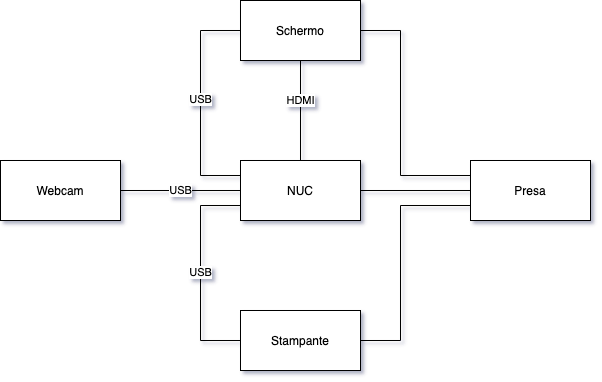
\includegraphics[width=0.7\textwidth]{img/cables_it.png}
                \caption{Schema dei vari collegamenti}
                \label{cables}
        \end{figure}
		
		
	\subsection{Avvio}
	
	\begin{enumerate}		
		\item Accendere l'interruttore principale dello schermo, posizionato vicino al connettore di alimentazione
		\item Premere il pulsante di accensione del NUC
		\item Premere per qualche secondo il tasto di accensione della stampante
		\item Quando si presenta la schermata di blocco di windows, trascinare l'immagine verso l'alto e inserire la password \texttt{usi-warpme} con l'aiuto della tastiera a schermo
		\item Il software dovrebbe avviarsi automaticamente. Qualora non fosse il caso, toccare due volte l'icona \texttt{WarpMe} sul Desktop
	\end{enumerate}	
		
		
		
\section{Utilizzo}

	\subsection{Scattare una foto}

		//TODO scattare foto e deformare
	
	
	\subsection{Esportazione}
	
		//TODO stampare o email
		
	
	
\section{Spegnimento}
	
		//TODO spegnimento
	
	
	
\section{Manutenzione}

	\subsection{Carta stampante}
	
		//TODO refill carta stampante, ref per ricambi
		
		
	\subsection{Inchiostro stampante}
	
		//TODO cambio cartuccia stampante, ref per ricambi
		
		
\section{Codice sorgente}

	Il codice sorgente si trova qui: \url{https://bitbucket.org/teseoch/image-morphing/}.
		
	
\end{document}